% ieeeaccess.cls reuses \year as a metadata setter. Preserve the TeX primitive
% so PGF/TikZ can initialize its deterministic machinery while loading.
\let\PSevenTeXYear\year
\documentclass{ieeeaccess}

% Shared packages and notation. Do not change IEEE Access class formatting here.
\usepackage{cite}
\usepackage{amsmath,amssymb,amsfonts}
\usepackage{graphicx}
\usepackage{textcomp}
\usepackage{bm}
\usepackage{booktabs}
\usepackage{array}
\usepackage{xcolor}
\usepackage[hidelinks]{hyperref}

\newtheorem{proposition}{Proposition}
\newtheorem{definition}{Definition}

\DeclareMathOperator*{\argmax}{arg\,max}
\DeclareMathOperator*{\argmin}{arg\,min}
\newcommand{\R}{\mathbb{R}}
\newcommand{\Pset}{\mathcal{P}}
\newcommand{\Hset}{\mathcal{H}}
\newcommand{\given}{\,|\,}

\newcommand{\ObservedPMUCount}{8}
\newcommand{\HiddenBusCount}{31}
\newcommand{\NominalTestCount}{100}
\newcommand{\BZeroTVE}{0.3402\%}
\newcommand{\BOneTVE}{0.009904\%}
\newcommand{\BTwoTVE}{0.009634\%}
\newcommand{\BTwoRelativeImprovement}{2.7\%}
\newcommand{\FunctionalSpearman}{0.5625}
\newcommand{\MismatchMainCount}{980}
\newcommand{\MismatchRefinementCount}{175}
\newcommand{\NetworkMismatchRatio}{16.99}
\newcommand{\OperatingMismatchRatio}{8.32}
\newcommand{\OnlineClosurePercent}{0.4\%}
\newcommand{\UtwoNLL}{-16.184}
\newcommand{\UtwoCoverageRe}{93.9\%}
\newcommand{\UtwoCoverageIm}{94.2\%}
\newcommand{\OriginalInnovationACF}{0.602}
\newcommand{\MeasurementGMInnovationACF}{0.540}
\newcommand{\MismatchUzeroCoverage}{92.9\%}
\newcommand{\MismatchUtwoCoverage}{47.5\%}
\newcommand{\AdequacyHalfAUROC}{0.901}
\newcommand{\AdequacyHalfAUPRC}{0.779}
\newcommand{\AdequacyMaxAUROC}{0.928}
\newcommand{\AdequacyMaxAUPRC}{0.787}
\newcommand{\NetworkFrozenTVE}{0.250430\%}
\newcommand{\NetworkOracleTVE}{0.002547\%}
\newcommand{\NetworkOnlineTVE}{0.251132\%}
\newcommand{\OperatingFrozenTVE}{0.122641\%}
\newcommand{\OperatingOracleTVE}{0.001006\%}
\newcommand{\OperatingOnlineTVE}{0.122381\%}
\newcommand{\CoupledFrozenTVE}{0.023615\%}
\newcommand{\CoupledOracleTVE}{0.000396\%}
\newcommand{\CoupledOnlineTVE}{0.023615\%}


\begin{document}
\history{}
\doi{}

\title{Physics-Informed State Reconstruction and Event-Source Inference From Sparse PMUs Under Limited Observability}
\author{\uppercase{Jorge Luis Mayorga Taborda}\authorrefmark{1}, \uppercase{Yessica Africano Rodriguez}\authorrefmark{1}, \uppercase{Masoud Barati}\authorrefmark{2}, \uppercase{Payman Dehghanian}\authorrefmark{3}, AND \uppercase{David Felipe Celeita Rodr\'iguez}\authorrefmark{4}}

\address[1]{Universidad de los Andes, Bogot\'a, Colombia}
\address[2]{Department of Electrical and Computer Engineering, University of Pittsburgh, Pittsburgh, PA, USA}
\address[3]{Department of Electrical and Computer Engineering, The George Washington University, Washington, DC, USA}
\address[4]{Faculty of Engineering, Universidad de La Sabana, Ch\'ia, Colombia}

\markboth{Mayorga Taborda \headeretal, Sparse-PMU State Reconstruction and Event-Source Inference}{Mayorga Taborda \headeretal, Sparse-PMU State Reconstruction and Event-Source Inference}

\hypersetup{
  pdftitle={From State Recoverability to Event-Source Diagnosability: Physics-Based Inference From Sparse PMUs},
  pdfauthor={Jorge Luis Mayorga Taborda; Yessica Africano Rodriguez; Masoud Barati; Payman Dehghanian; David Felipe Celeita Rodriguez},
  pdfsubject={Sparse-PMU state recoverability, event-source diagnosability, and physics-based inference},
  pdfkeywords={dynamic state estimation, functional observability, phasor measurement units, physics-informed inference, source localization}
}

\begin{abstract}
Accurate recovery of an unmeasured voltage field does not imply that sparse phasor measurement units (PMUs) can identify the physical source of a disturbance. We formalize this distinction in a hybrid differential-algebraic model that separates hidden state, physical intervention, and measurement integrity. Functional observability characterizes the requested voltage field; a nuisance-profiled separation margin characterizes event-source diagnosability. Evidence comes from two frozen IEEE 39-bus campaigns using the same eight PMU buses but different simulators and contracts. On 100 PowerDynamics nonlinear test trajectories, a causal Kalman estimator reduces mean hidden-bus relative complex-voltage error from \BZeroTVE{} to \BTwoTVE{}; a preregistered functional residual correlates with bus-level error ($\rho=\FunctionalSpearman$). A measurement-only regularized physical recentering closes \EZeroHClosureHalf{}--\EZeroHClosureMax{} of the nominal-center error gap on 60 operating-point-shifted plants despite nuisance-information rank \EZeroHRank{}/\EZeroHDimension{}. On a separate 690-trajectory ANDES event bank, a physics-guided hierarchy attains detection F1 \LegacyEventDetectionFOne{}, event macro-F1 \LegacyEventMacroFOne{}, and physical-source Top-1 \LegacyPhysicalTopOne{} when sources are represented during training. Under complete source holdout, only \HeldSourceCorrect{} of \HeldSourceDecisions{} decisions are correct. The evidence establishes sparse-PMU state recoverability under the tested conditions and rejects source-generalization for the learned baseline; the proposed end-to-end joint estimator remains unvalidated.
\end{abstract}

\begin{keywords}
dynamic state estimation, event detection, functional observability, limited observability, phasor measurement units, physics-informed inference, source localization.
\end{keywords}

\titlepgskip=-21pt
\maketitle

\section{Introduction}
\label{sec:introduction}

\PARstart{P}{hasor} measurement units (PMUs) reveal electromechanical transients through synchronized voltage and current phasors, yet only a fraction of the buses and branches in a transmission network are normally instrumented \cite{phadke2008synchronized,zhao2019dse}. A disturbance may therefore originate outside the measured region, alter hidden voltages, and propagate to the available devices. At the same time, a missing frame or corrupted channel can resemble a physical transient. A useful diagnosis must answer three distinct questions: what is the network state, which physical or measurement event is present, and where did each applicable event originate?

Strong prior methods solve important subsets of this problem. Dynamic estimators combine physical models with synchrophasors \cite{zhao2019dse,katanic2024recursive}; sparse-PMU classifiers identify events and faulted assets \cite{pandey2020realtime,yildiz2024few}; and recent learning systems reconstruct hidden trajectories before localization or estimate state and attack location from partial observations \cite{rimkus2025gnn,zhai2025partial}. These results make a broad ``joint inference'' novelty claim untenable. The unresolved contract considered here is narrower: causal inference in an under-observed transmission system when physical interventions and measurement-integrity failures can coexist, the source asset may be absent from source-labeled training, and the sensing geometry may make two candidate sources physically indistinguishable.

This distinction matters because event recognition, state reconstruction, and source localization have different information requirements. A generation change can be detected throughout the network while its source remains ambiguous. A dropped PMU identifies an integrity location directly but removes information needed to localize a simultaneous physical event. Likewise, a state estimate can have low point error although the nuisance intervention is not uniquely identifiable. Treating all three tasks as one multiclass label hides these differences and encourages scores whose denominator does not match the claimed capability.

We represent a physical event as an intervention hypothesis $h=(c,\ell,\tau,\gamma)$ containing family, source, onset, and magnitude, and represent measurement integrity separately through a time-varying availability operator and an additive corruption process. Each physical candidate produces a counterfactual DAE response. Candidate comparison profiles the admissible initial-state and integrity nuisance directions. The resulting separation margin exposes source pairs that the available PMUs cannot distinguish and motivates a candidate set or abstention instead of a forced source.

The empirical record currently contains two complementary, frozen campaigns. The PowerDynamics campaign audits an IEEE 39-bus hybrid DAE, reconstructs 31 hidden complex bus voltages from eight voltage/current PMUs, and studies model mismatch and physical recentering. The separate ANDES campaign contains \LegacyEventTrajectories{} trajectories spanning eight abnormal classes plus normal operation and evaluates a physics-guided hierarchical ExtraTrees baseline. The two campaigns share PMU buses and a network family, but not simulator semantics, state coordinates, or split contracts; their metrics are never pooled. The event study is presented as a baseline and failure analysis, not as evidence that the proposed joint posterior has already been executed.

The paper makes four contributions.
\begin{enumerate}
  \item We formulate sparse-PMU monitoring as joint inference over hidden state, physical intervention, physical source, and measurement integrity. The eight event labels are mapped to composable physical and integrity variables rather than treated as eight unrelated phenomena.
  \item We distinguish functional observability of the requested voltage field from event-source diagnosability. A finite-horizon affine-manifold distance gives a local theoretical limit: intersecting hypothesis manifolds admit nuisance configurations that no decision rule can distinguish uniformly.
  \item We consolidate two audited evidence lines. On the state campaign, a preregistered structural residual predicts bus-level reconstruction difficulty and measurement-only regularized physical recentering recovers operating-point-shifted voltages. On the event campaign, multiscale and spatial features improve known-source localization, but complete source holdout collapses to \HeldSourceCorrect{}/\HeldSourceDecisions{} exact decisions.
  \item We define the reproducible comparison required for the next joint experiment: learned-only diagnosis, physics-only hypothesis inference, physics plus learned residual discrepancy, and diagnosability-aware inference with abstention, all evaluated on source-disjoint parents with explicit alarm exposure and PMU loss/join conditions.
\end{enumerate}

The strongest result is also the main limitation. The state component is accurate under the tested nominal and operating-point-shift contracts, and the known-source event baseline attains detection F1 \LegacyEventDetectionFOne{} and event macro-F1 \LegacyEventMacroFOne{}. Yet source localization does not transfer to assets excluded from training. The current manuscript therefore establishes the mathematical and empirical boundary that a joint physics-informed method must cross; it does not convert a proposed end-to-end estimator into a completed result.

\begin{figure*}[t]
\centering
\resizebox{\textwidth}{!}{\begin{tikzpicture}[
  x=1cm,y=1cm,
  font=\sffamily\scriptsize,
  >=Latex,
  box/.style={draw=black!55,rounded corners=2pt,thick,align=center,
    minimum height=0.72cm,inner sep=3pt,fill=white},
  state/.style={box,draw=accessblue!75!black,fill=accessblue!8},
  event/.style={box,draw=orange!78!black,fill=orange!9},
  loadcase/.style={box,draw=green!55!black,fill=green!7},
  pending/.style={box,draw=purple!72!black,densely dashed,fill=purple!5},
  arr/.style={->,thick,draw=black!60,rounded corners=2pt},
  pendingarr/.style={->,thick,densely dashed,draw=purple!72!black,rounded corners=2pt},
  lane/.style={font=\sffamily\tiny\bfseries,anchor=east,align=right}
]

% Column headings make the contract readable before the individual boxes.
\foreach \x/\txt in {0.95/OBSERVATIONS,3.72/PHYSICAL MODEL,6.72/INFERENCE,9.82/EVIDENCE,13.10/OUTPUT}{
  \node[font=\sffamily\tiny\bfseries,text=black!58] at (\x,3.48) {\txt};
}

\node[state,text width=2.05cm,minimum height=1.15cm] (pmu) at (0.95,1.48)
  {PMU frame at $k$\\$\bm y_k=\{V,I,f\}$\\$\bm M_k,\bm b_k$, quality flags};

\node[state,text width=2.10cm] (dae) at (3.72,2.45)
  {Network and DAE model\\$\bm f,\bm g,\bm h_{\mathcal P}$};
\node[event,text width=2.10cm] (bank) at (3.72,0.45)
  {Physical hypothesis bank\\$h=(c,\ell,\tau,\gamma)$};

\node[state,text width=2.25cm] (statefit) at (6.72,2.45)
  {Causal state estimator\\frozen B0--B3 tests};
\node[pending,text width=2.38cm,minimum height=0.90cm] (jointfit) at (6.72,1.20)
  {Candidate-conditioned fit\\state and integrity nuisance};
\node[loadcase,text width=2.25cm] (loadfit) at (6.72,-0.05)
  {Load tangent\\and fitted noise};

\node[pending,text width=2.30cm,minimum height=0.90cm] (compare) at (9.82,1.20)
  {Profiled candidate evidence\\$D_{ij},\ p(h\mid\bm y_{0:k})$};
\node[loadcase,text width=2.22cm] (loadpost) at (9.82,-0.05)
  {Closed evaluated bank\\$H_0$ and 16 load buses};

\node[state,text width=2.32cm] (stateout) at (13.10,2.45)
  {Hidden-voltage estimate\\$\widehat{\bm z}_{\mathcal U,k},\bm\Sigma_{z,k}$};
\node[event,text width=2.32cm] (eventout) at (13.10,1.05)
  {Event, source, integrity\\$\widehat c_k,\widehat\ell_k,\widehat q_k$};
\node[pending,text width=1.55cm] (abstain) at (15.55,1.05)
  {candidate set\\or abstain};

% Three distinct lanes: evaluated state, pending joint inference, and evaluated load-only inference.
\node[lane,text=accessblue!80!black] at (-0.35,2.45) {evaluated\\state lane};
\node[lane,text=purple!78!black] at (-0.35,1.20) {joint lane\\not evaluated};
\node[lane,text=green!48!black] at (-0.35,-0.05) {evaluated\\load lane};

\begin{scope}[on background layer]
  \draw[arr,draw=accessblue!72!black] ($(pmu.east)+(0,0.40)$) -- (dae.west);
  \draw[arr,draw=accessblue!72!black] (dae) -- (statefit);
  \draw[arr,draw=accessblue!72!black] (statefit) -- (stateout);

  \draw[pendingarr] (pmu.east) -- (jointfit.west);
  \draw[pendingarr] (dae.south) -- (jointfit.north);
  \draw[pendingarr] (bank.north) -- (jointfit.south);
  \draw[pendingarr] (jointfit) -- (compare);
  \draw[pendingarr] (compare.east) -- (eventout.west);
  \draw[pendingarr] (compare.north east) -| (stateout.south);

  \draw[arr,draw=green!48!black] (pmu.south) -- (0.95,-0.62) -- (5.24,-0.62) |- (loadfit.west);
  \draw[arr,draw=green!48!black] (bank) -- (loadfit);
  \draw[arr,draw=green!48!black] (loadfit) -- (loadpost);
  \draw[arr,draw=green!48!black] (loadpost.east) -| (eventout.south);
  \draw[pendingarr] (eventout) -- (abstain);
\end{scope}

\node[font=\sffamily\tiny,text=black!58,anchor=west] at (1.55,-0.92)
  {solid blue/green: executed evidence};
\node[font=\sffamily\tiny,text=purple!78!black,anchor=west] at (6.45,-0.92)
  {purple dashed: proposed multi-family joint path};
\node[font=\sffamily\tiny,text=orange!80!black,anchor=west] at (12.55,-0.92)
  {orange: physical/integrity decision};
\end{tikzpicture}
}
\caption{Joint inference contract. The physical model generates candidate state and PMU responses, while availability and quality govern which residuals are admissible. Physical interventions and measurement-integrity failures remain separate latent variables. The rightmost outputs distinguish hidden-state uncertainty from event/source ambiguity and permit a candidate set instead of a forced source. Solid arrows describe the proposed online information flow; this paper validates its state-estimation and historical diagnosis components separately.}
\label{fig:joint-architecture}
\end{figure*}

The remainder of the paper reviews the closest estimation and localization contracts, defines the hybrid DAE and eight event labels, derives the observability and diagnosability limits, specifies the estimator hierarchy, documents both evidence campaigns, and reports the validated results and unresolved joint-inference gate.

\section{Related Work and Research Gap}
\label{sec:related-work}

% Drafted in the research-gap commit.

\section{Joint State, Event, and Source Problem}
\label{sec:problem-formulation}

\subsection{Hybrid DAE and Electrical Measurement Model}

Let $\bm x(t)\in\mathbb R^{n_x}$ denote differential states, $\bm z(t)\in\mathbb R^{n_z}$ algebraic states, $\bm u(t)$ scheduled inputs, $\bm q(t)$ network configuration, and $\bm\theta$ physical parameters. A physical intervention $\bm a_h(t)$ is indexed by hypothesis
\begin{equation}
 h=(c,\ell,\tau,\gamma,\bm d), \qquad h\in\mathcal H,
 \label{eq:physical-hypothesis}
\end{equation}
where $c$ is event family, $\ell$ is a bus or branch source, $\tau$ is onset, $\gamma$ is severity, and $\bm d$ describes the allowed temporal profile. The plant is
\begin{align}
 \dot{\bm x}(t)&=\bm f\!\left(\bm x,\bm z,\bm u,\bm q,\bm a_h;\bm\theta\right)+\bm w_x(t), \label{eq:dae-dynamic}\\
 \bm 0&=\bm g\!\left(\bm x,\bm z,\bm u,\bm q,\bm a_h;\bm\theta\right), \label{eq:dae-algebraic}\\
 \bm y_k&=\bm M_k\!\left[\bm h_{\mathcal P_k}(\bm x_k,\bm z_k,\bm q_k;\bm\theta)+\bm b_k\right]+\bm v_k. \label{eq:dae-measurement}
\end{align}
Here $\bm M_k$ selects the channels that are available at time $k$, $\bm b_k$ is a measurement-corruption process, and $\bm v_k$ is measurement noise. A dropout changes $\bm M_k$; bad data change $\bm b_k$; neither is a physical input to \eqref{eq:dae-dynamic}--\eqref{eq:dae-algebraic}. This separation permits a physical event and a measurement failure to coexist.

The algebraic network core is
\begin{equation}
 \bm I=\bm Y_{\mathrm{bus}}(\bm q,\bm\theta)\bm V,
 \qquad S_i=P_i+\mathrm jQ_i=V_i I_i^{*}. \label{eq:network-core}
\end{equation}
Writing $\bm Y_{\mathrm{bus}}=\bm G+\mathrm j\bm B$ and $V_i=|V_i|e^{\mathrm j\vartheta_i}$ gives
\begin{align}
 P_i&=|V_i|\sum_j|V_j|\!\left[G_{ij}\cos\vartheta_{ij}+B_{ij}\sin\vartheta_{ij}\right], \label{eq:ac-p}\\
 Q_i&=|V_i|\sum_j|V_j|\!\left[G_{ij}\sin\vartheta_{ij}-B_{ij}\cos\vartheta_{ij}\right], \label{eq:ac-q}
\end{align}
where $\vartheta_{ij}=\vartheta_i-\vartheta_j$. A line outage changes the branch primitives and therefore $\bm Y_{\mathrm{bus}}$; a bus fault adds a shunt-admittance intervention; generation and load changes modify the appropriate active/reactive injection equations. For a PMU at one terminal of branch $(i,j)$,
\begin{equation}
 I_{ij}=Y_{ff,ij}V_i+Y_{ft,ij}V_j,
 \qquad I_{ji}=Y_{tf,ij}V_i+Y_{tt,ij}V_j. \label{eq:terminal-current}
\end{equation}
The orientation, transformer tap, line charging, and shunt convention in \eqref{eq:terminal-current} are part of the inference contract; replacing terminal current with bus-injection current changes the likelihood.

\subsection{Sparse PMUs and Requested State Function}

Both evidence campaigns use PMU buses
\begin{equation}
 \mathcal P=\{2,5,6,10,19,22,29,39\},\qquad |\mathcal P|=8. \label{eq:pmu-set}
\end{equation}
The unobserved set is $\mathcal U=\{1,\ldots,39\}\setminus\mathcal P$, with $|\mathcal U|=31$. The state-estimation campaign stacks rectangular voltage and controlled terminal-current components,
\begin{equation}
 \bm y_{\mathcal P,k}=\operatorname{col}_{p\in\mathcal P}
 [\Re V_{p,k},\Im V_{p,k},\Re I_{p\ell,k},\Im I_{p\ell,k}], \label{eq:pmu-vector}
\end{equation}
and requests the hidden complex-voltage function
\begin{equation}
 \bm z_{\mathcal U,k}=\operatorname{col}_{i\in\mathcal U}[\Re V_{i,k},\Im V_{i,k}]\in\mathbb R^{62}. \label{eq:hidden-target}
\end{equation}
The event campaign also uses voltage angle, frequency, availability, and, in its longer-window implementation, current and ROCOF. Measurement semantics are kept campaign-specific rather than declaring channels equivalent across simulators.

\subsection{Eight Event Labels as Composable States}

Table~\ref{tab:event-ontology} defines the eight abnormal labels in the historical event bank. The scientific variables are not the label numbers. Classes 1--4 are single physical interventions; classes 5 and 7 are measurement-integrity states; classes 6 and 8 are compositions. Class 8 is a prescribed mixed event in the available simulations, not evidence of open-set recognition.

\begin{table*}[t]
\caption{Event ontology and historical ANDES inventory. Each source configuration has five replicas. ``Physical source'' and ``integrity source'' are separate outputs.}
\label{tab:event-ontology}
\centering
\footnotesize
\begin{tabularx}{\textwidth}{@{}cXlllr@{}}
\toprule
ID & Operational meaning & Physical intervention $c$ & Physical source $\ell$ & Integrity state/source & Records \\
\midrule
0 & Normal operation & none & none & nominal & 5 \\
1 & Bus fault & fault admittance & bus & nominal & 195 \\
2 & Line outage & topology removal & branch & nominal & 170 \\
3 & Generation change & active/reactive injection & generator bus & nominal & 50 \\
4 & Load change & active/reactive withdrawal & load bus & nominal & 90 \\
5 & Missing data & none & none & dropout / PMU & 40 \\
6 & Generation change with missing data & generation change & generator bus & dropout / PMU & 50 \\
7 & Bad data & none & none & corruption / PMU channel & 40 \\
8 & Prescribed mixed disturbance & generation plus load changes & declared generator bus & measurement disturbance / PMU & 50 \\
\midrule
 & Total & & & & 690 \\
\bottomrule
\end{tabularx}
\end{table*}

The internal decision at time $k$ is
\begin{equation}
 \left(\widehat{\bm z}_{\mathcal U,k},\bm\Sigma_{z,k},
 \widehat c_k,\widehat\ell^{\mathrm{phys}}_k,
 \widehat m_k,\widehat\ell^{\mathrm{meas}}_k,\mathcal C_k\right),
 \label{eq:joint-output}
\end{equation}
where $m_k$ denotes the integrity state and $\mathcal C_k\subseteq\mathcal H$ is a credible candidate set. A location is empty when it does not apply. The candidate set is required because limited observability can make a forced Top-1 decision scientifically unjustified.

\subsection{Correctness and Evaluation Units}

State accuracy uses hidden-bus total vector error
\begin{equation}
 \operatorname{TVE}^{(r)}=\frac{1}{T_r|\mathcal U|}
 \sum_{k=1}^{T_r}\sum_{i\in\mathcal U}
 \frac{|\widehat V_{i,k}-V_{i,k}|}{\max(|V_{i,k}|,\epsilon)}, \label{eq:tve}
\end{equation}
reported as a percentage. Event detection, event-family macro-F1, exact physical Top-1/Top-3, and integrity-source Top-1 use their own declared populations. The joint correctness indicator is one only when every applicable component of \eqref{eq:joint-output} is correct; a correct event family cannot conceal a wrong source. Confidence intervals use an independently generated trajectory, event parent, or rebuilt plant as the statistical unit, never individual 30-Hz samples.

The causal contract permits only $\bm y_{0:k}$ at time $k$. A fixed-lag smoother, complete-window statistic, or centered temporal feature is retrospective and is labeled accordingly. Source generalization requires that physical source $\ell$ be absent from all source-labeled training and tuning, not merely that the test trajectory use a new random seed.

\section{Functional Observability of the Hidden Voltage Field}
\label{sec:functional-observability}

\subsection{Local Reduced Model}

Linearizing the index-reduced DAE around a verified equilibrium and sampling at $\Delta t=1/30$~s gives
\begin{align}
 \delta\bm x_{k+1} &= \bm A_d\delta\bm x_k+\bm w_k, \label{eq:local-state}\\
 \delta\bm y_k &= \bm C\delta\bm x_k+\bm v_k, \label{eq:local-output}\\
 \delta\bm z_{\mathcal U,k} &= \bm L_{\mathcal U}\delta\bm x_k. \label{eq:local-target}
\end{align}
Here $\delta\bm x_k\in\mathbb R^{114}$ contains the reduced differential coordinates, $\bm C$ maps them to the 32 voltage/current PMU channels, and $\bm L_{\mathcal U}$ maps them to the 62 rectangular hidden-voltage components. These matrices are local: their validity can degrade when the operating point or physical parameters move away from the linearization point.

For a horizon of $N$ transitions, define
\begin{equation}
 \mathcal O_N=\operatorname{col}\left(\bm C,\bm C\bm A_d,\ldots,\bm C\bm A_d^N\right). \label{eq:observability-matrix}
\end{equation}
Full-state observability requires $\operatorname{rank}(\mathcal O_N)=114$. Hidden-voltage reconstruction requires a weaker, target-specific condition \cite{fernando2010functional,zhang2025functional}.

\begin{proposition}[Finite-horizon functional reconstruction]
\label{prop:functional-reconstruction}
For the noise-free system \eqref{eq:local-state}--\eqref{eq:local-target}, the initial target $\bm L_{\mathcal U}\delta\bm x_0$ is uniquely determined by the output sequence through horizon $N$ if and only if
\begin{equation}
 \ker\mathcal O_N\subseteq\ker\bm L_{\mathcal U}. \label{eq:functional-condition}
\end{equation}
Equivalently, there exists a matrix $\bm M_N$ such that $\bm L_{\mathcal U}=\bm M_N\mathcal O_N$.
\end{proposition}

\IEEEproof
Two initial states produce the same output history exactly when their difference belongs to $\ker\mathcal O_N$. Their target values agree for every such pair exactly when that difference also belongs to $\ker\bm L_{\mathcal U}$, proving \eqref{eq:functional-condition}. In finite-dimensional spaces, $\ker\mathcal O_N\subseteq\ker\bm L_{\mathcal U}$ is equivalent to the rows of $\bm L_{\mathcal U}$ lying in the row space of $\mathcal O_N$, which yields $\bm L_{\mathcal U}=\bm M_N\mathcal O_N$.
\endIEEEproof

Proposition~\ref{prop:functional-reconstruction} is a standard linear-algebraic characterization, not a novelty claim. Its role is to define the correct structural object for the tested output. It also makes clear that a low full-state rank does not by itself preclude accurate recovery of $\bm z_{\mathcal U}$.

\subsection{Numerical Functional Residual}

Exact rank statements are fragile under floating-point scaling, so the experiment uses the observable-subspace projector
\begin{equation}
 \bm\Pi_N=\mathcal O_N^{\dagger}\mathcal O_N \label{eq:observable-projector}
\end{equation}
and the target residual
\begin{equation}
 r_F(N)=\left\|\bm L_{\mathcal U}(\bm I-\bm\Pi_N)\right\|_F. \label{eq:functional-residual}
\end{equation}
For hidden bus $i$, the corresponding two-row map $\bm L_i$ gives
\begin{equation}
 r_{F,i}(N)=\left\|\bm L_i(\bm I-\bm\Pi_N)\right\|_F. \label{eq:bus-functional-residual}
\end{equation}
A smaller value means that fewer target directions project onto the numerically unobservable state subspace. It is a structural diagnostic at the frozen equilibrium, not an empirical error or a probabilistic confidence interval.

The projector is obtained from the eigendecomposition of $\mathcal O_N^{\mathsf T}\mathcal O_N$ using a fixed relative eigenvalue tolerance of $10^{-9}$. Horizons $N\in\{0,3,10,30,60,120,180\}$ are evaluated. The $N=180$ bus-level residuals and their ranking were exported before nonlinear reconstruction was scored. This preregistration permits a genuine theory-to-evidence test: the paper correlates $r_{F,i}(180)$ with per-bus TVE rather than defining the diagnostic after seeing the error pattern.

The same Gramian produces a trace-style noise amplification diagnostic under independent rectangular-voltage noise with standard deviation $10^{-3}$~pu. Because this bound depends on the local linearization and numerical rank tolerance, it is reported as structural context rather than as estimator performance.

\subsection{Event-Source Diagnosability Under Nuisance State}

Functional observability concerns a state function; source localization concerns separation among interventions. Linearize candidate $h$ over a horizon of $H$ samples:
\begin{align}
 \delta\bm x_{k+1}&=\bm A_k\delta\bm x_k+\bm B_{h,k}\bm d_{h,k}+\bm w_k, \label{eq:event-linear-state}\\
 \delta\bm y_k&=\bm C_k\delta\bm x_k+\bm E_k\bm b_k+\bm v_k. \label{eq:event-linear-output}
\end{align}
After stacking the available channels selected by $\bm M_k$,
\begin{equation}
 \bm Y_H=\mathcal O_H\delta\bm x_0+\bm s_{h,H}+\mathcal E_H\bm B_H+\bm\varepsilon_H, \label{eq:stacked-hypothesis}
\end{equation}
where $\bm s_{h,H}$ is the candidate physical response, $\mathcal O_H$ is the time-varying observability matrix, and $\mathcal E_H\bm B_H$ represents admissible integrity corruption. Let $\bm R_H$ be the stacked noise covariance. To avoid mistaking an uncertain initial condition for an event, define the $\bm R_H^{-1}$-orthogonal nuisance projector
\begin{equation}
 \bm P_{\mathcal O}^{\perp}=\bm I-\mathcal O_H
 (\mathcal O_H^{\mathsf T}\bm R_H^{-1}\mathcal O_H)^{\dagger}
 \mathcal O_H^{\mathsf T}\bm R_H^{-1}. \label{eq:nuisance-projector}
\end{equation}
The usable signature is $\widetilde{\bm s}_{h,H}=\bm P_{\mathcal O}^{\perp}\bm s_{h,H}$. For candidates $i$ and $j$ with equal projected covariance, their local pairwise information is
\begin{equation}
 D_{ij}^{(\mathcal P)}(H)=\frac{1}{2}
 (\widetilde{\bm s}_{i,H}-\widetilde{\bm s}_{j,H})^{\mathsf T}
 \bm R_{\perp}^{\dagger}
 (\widetilde{\bm s}_{i,H}-\widetilde{\bm s}_{j,H}), \label{eq:pairwise-information}
\end{equation}
with $\bm R_{\perp}=\bm P_{\mathcal O}^{\perp}\bm R_H(\bm P_{\mathcal O}^{\perp})^{\mathsf T}$. This is the Gaussian mean-separation term after removing initial-state nuisance. It is not a new divergence.

\begin{proposition}[Local indistinguishability]
\label{prop:source-indistinguishability}
Assume the linearized model \eqref{eq:stacked-hypothesis}, equal prior probability, equal projected covariance, and no integrity pattern that differentiates candidates $i$ and $j$. If $D_{ij}^{(\mathcal P)}(H)=0$, then the projected measurement distributions under $i$ and $j$ are identical. No decision rule based on the stated PMU history can attain an average error below $1/2$ for this pair.
\end{proposition}

\IEEEproof
Equation \eqref{eq:pairwise-information} is zero exactly when the two projected Gaussian means coincide on the support of $\bm R_{\perp}$. Equal covariance then makes the distributions identical. With equal priors, every measurable decision rule assigns the same observation law under both hypotheses, so its two conditional error probabilities sum to one.
\endIEEEproof

\begin{corollary}[Information cannot decrease when an independent PMU joins]
\label{cor:pmu-additivity}
If an added PMU block is conditionally independent of the existing measurements given each hypothesis and has a correctly specified covariance, then
\begin{equation}
 D_{ij}^{(\mathcal P\cup\{p\})}(H)=D_{ij}^{(\mathcal P)}(H)+D_{ij}^{(p)}(H)\ge D_{ij}^{(\mathcal P)}(H). \label{eq:information-additivity}
\end{equation}
\end{corollary}

The corollary follows from additivity of Gaussian log-likelihood ratios. It gives a theoretical upper direction, not a guarantee that an arbitrary learned classifier improves when a PMU is added. Model error, dependence, or poor normalization can violate the assumptions.

\begin{figure}[t]
\centering
\resizebox{\columnwidth}{!}{\begin{tikzpicture}[x=1cm,y=1cm,font=\sffamily\scriptsize,>=Latex]
% Linear candidate sets and their nonlinear remainder tubes.
\fill[accessblue!10] (-0.10,-0.02) -- (3.82,0.98) -- (3.82,1.34) -- (-0.10,0.34) -- cycle;
\draw[accessblue!75!black,very thick] (0.00,0.16) -- (3.72,1.12);
\draw[accessblue!75!black,densely dashed,thick]
  (0.00,0.10) .. controls (1.15,0.55) and (2.45,0.50) .. (3.72,1.24);
\node[text=accessblue!80!black,anchor=south west] at (0.10,0.42)
  {$\mathcal M_i^{\mathrm{lin}}$};

\fill[orange!12] (-0.10,2.16) -- (3.82,3.16) -- (3.82,3.52) -- (-0.10,2.52) -- cycle;
\draw[orange!85!black,very thick] (0.00,2.34) -- (3.72,3.30);
\draw[orange!85!black,densely dashed,thick]
  (0.00,2.45) .. controls (1.30,2.54) and (2.35,3.28) .. (3.72,3.18);
\node[text=orange!85!black,anchor=south west] at (0.10,2.60)
  {$\mathcal M_j^{\mathrm{lin}}$};

\coordinate (pi) at (2.02,0.68);
\coordinate (pj) at (1.52,2.73);
\fill[accessblue!80!black] (pi) circle (1.5pt);
\fill[orange!85!black] (pj) circle (1.5pt);
\draw[<->,very thick,green!50!black] (pi) -- (pj)
  node[midway,right=2pt,align=left] {$d_{ij}^{\mathrm{lin}}$\\profiled distance};

\draw[<->,thick,purple!75!black] (3.42,1.24) -- (3.42,3.08)
  node[midway,right=2pt] {$d_{ij}^{\mathrm{nl}}$};

\node[draw=black!30,rounded corners=2pt,fill=white,align=left,inner sep=4pt]
  at (5.55,2.55)
  {$d_{ij}^{\mathrm{nl}}\geq$\\$[d_{ij}^{\mathrm{lin}}-\epsilon_i(r)-\epsilon_j(r)]_+$};
\node[draw=black!30,rounded corners=2pt,fill=white,align=left,inner sep=4pt]
  at (5.55,0.80)
  {solid: affine model\\dashed: nonlinear response\\shading: remainder bound};
\end{tikzpicture}
}
\caption{Local source-diagnosability geometry. Components within the initial-state response subspace are nuisance; only the projected difference separates two physical-source candidates. Coincident projected signatures imply the lower bound in Proposition~\ref{prop:source-indistinguishability}.}
\label{fig:diagnosability-geometry}
\end{figure}

For a source posterior $p(h\mid\bm y_{0:k})$, define the smallest candidate set satisfying
\begin{equation}
 \mathcal C_k(\alpha)=\argmin_{\mathcal C\subseteq\mathcal H}
 \left\{|\mathcal C|:\sum_{h\in\mathcal C}p(h\mid\bm y_{0:k})\ge1-\alpha\right\}. \label{eq:candidate-set}
\end{equation}
A diagnosability-aware system abstains from exact Top-1 when $|\mathcal C_k|>1$ or when the minimum information to a competing hypothesis falls below a development-set threshold. The pending joint experiment must test whether \eqref{eq:pairwise-information} predicts candidate-set size, posterior entropy, and source-resolution delay under PMU loss/join. The current event bank has not yet supplied that evidence.

\section{Local Physics-Based Estimation and Diagnostics}
\label{sec:estimation}

\subsection{Nominal Estimator Hierarchy}

All estimators use the same equilibrium $\bm y_0$, hidden-voltage center $\bm z_{\mathcal U,0}$, sampled dynamics $\bm A_d$, PMU map $\bm C$, and hidden-output map $\bm L_{\mathcal U}$. This shared model isolates the value of measurement updating and temporal propagation.

The equilibrium baseline B0 returns
\begin{equation}
 \widehat{\bm z}^{\mathrm{B0}}_{\mathcal U,k}=\bm z_{\mathcal U,0}. \label{eq:b0}
\end{equation}
It measures how much of the score can be obtained by remaining at the nominal power-flow solution.

The snapshot estimator B1 computes the minimum-variance linear update independently at every frame,
\begin{align}
 \bm K_{\mathrm{WLS}}&=\bm P_0\bm C^{\mathsf T}
 \left(\bm C\bm P_0\bm C^{\mathsf T}+\bm R\right)^{-1}, \label{eq:wls-gain}\\
 \widehat{\delta\bm x}^{\mathrm{B1}}_k&=\bm K_{\mathrm{WLS}}(\bm y_k-\bm y_0), \qquad
 \widehat{\bm z}^{\mathrm{B1}}_{\mathcal U,k}=\bm z_{\mathcal U,0}+\bm L_{\mathcal U}\widehat{\delta\bm x}^{\mathrm{B1}}_k. \label{eq:wls-update}
\end{align}
B1 uses network-constrained cross-covariance but no state carried from frame $k-1$.

The causal Kalman estimator B2 applies the classical linear-Gaussian recursion \cite{kalman1960}:
\begin{align}
 \widehat{\bm x}_{k|k-1}&=\bm A_d\widehat{\bm x}_{k-1|k-1}, \label{eq:kf-predict-state}\\
 \bm P_{k|k-1}&=\bm A_d\bm P_{k-1|k-1}\bm A_d^{\mathsf T}+\bm Q, \label{eq:kf-predict-cov}\\
 \bm\nu_k&=(\bm y_k-\bm y_0)-\bm C\widehat{\bm x}_{k|k-1}, \label{eq:innovation}\\
 \bm S_k&=\bm C\bm P_{k|k-1}\bm C^{\mathsf T}+\bm R, \label{eq:innovation-cov}\\
 \bm K_k&=\bm P_{k|k-1}\bm C^{\mathsf T}\bm S_k^{-1}, \label{eq:kf-gain}\\
 \widehat{\bm x}_{k|k}&=\widehat{\bm x}_{k|k-1}+\bm K_k\bm\nu_k. \label{eq:kf-update}
\end{align}
The covariance update uses the Joseph form. The hidden estimate is $\bm z_{\mathcal U,0}+\bm L_{\mathcal U}\widehat{\bm x}_{k|k}$. B2 is causal because only $\bm y_{0:k}$ enters the result at $k$.

B3 is an exact fixed-lag Gaussian smoother, following the linear Gaussian backward-recursion principle in \cite{rauch1965smoothing}, evaluated at lags $\ell\in\{0,1,3,5,10,15,30,60\}$ frames. It uses measurements through $k+\ell$ to refine the estimate at $k$ and is therefore retrospective by $\ell/30$ seconds. Dense and cached implementations agree numerically on representative lags. B3 tests whether temporal information beyond the causal update improves the hidden-voltage target; it is not used to support a real-time claim.

\subsection{Marginal Calibration and Colored Discrepancy}

For the hidden two-component voltage error at bus $i$, B2 provides
\begin{equation}
 \bm\Sigma_{i,k}=\bm L_i\bm P_{k|k}\bm L_i^{\mathsf T}. \label{eq:hidden-covariance}
\end{equation}
The original covariance is U0. A two-block temperature model U2 is fitted on an independent calibration split:
\begin{equation}
 \bm\Sigma^{\mathrm{U2}}_{i,k}=\bm T\bm\Sigma_{i,k}\bm T^{\mathsf T},\qquad
 \bm T=\operatorname{diag}(\sqrt{\tau_{\Re}},\sqrt{\tau_{\Im}}). \label{eq:temperature}
\end{equation}
The temperatures minimize Gaussian negative log likelihood (NLL) on calibration data and are frozen before TEST. Coverage, NLL, normalized innovation squared (NIS), and temporal innovation correlation are reported separately; nominal marginal coverage alone is not called complete calibration.

The residual study considers a latent Gauss--Markov process
\begin{equation}
 \bm c_{k+1}=\bm F_c\bm c_k+\bm\eta_k. \label{eq:discrepancy-state}
\end{equation}
In D2-M, $\bm c_k$ enters the PMU measurement residual through a calibration-fitted low-rank basis. In D2-P, it enters a sparse physical process dictionary. Basis, rank, $\bm F_c$, and latent covariance are selected using calibration records only. The experiment asks whether the observed low-rank structure improves reconstruction, hidden uncertainty, or innovation whiteness. It does not assume that a lower innovation autocorrelation is sufficient.

\subsection{Model-Adequacy Statistic and Recentring Ablations}

Let $\bm\mu_{\nu}$ and $\bm\Sigma_{\nu}$ be the mean and shrunk covariance of B2 innovations on the nominal calibration set. The per-frame adequacy statistic is the five-frame trailing mean of
\begin{equation}
 a_k=(\bm\nu_k-\bm\mu_{\nu})^{\mathsf T}\bm\Sigma_{\nu}^{-1}(\bm\nu_k-\bm\mu_{\nu}). \label{eq:adequacy-score}
\end{equation}
Mismatch labels and hidden truth do not enter \eqref{eq:adequacy-score}; hidden truth is used only after inference to label frames whose hidden TVE exceeds the frozen evaluation threshold. AUROC and AUPRC therefore measure whether observed innovations anticipate unacceptable hidden error, not whether the detector identifies a mismatch family.

Two evaluation-only or adaptive variants diagnose the failure mechanism. R1 replaces the nominal equilibrium with the true plant equilibrium and is explicitly oracle. R2-A estimates an eight-dimensional grouped observed-bus voltage offset using a 60-frame trailing window, nominal matrices, ridge regularization, and only PMU measurements. It is a preregistered linearized static-MAP proxy, not a nonlinear AC power-flow or KKT solve. Its center/state cross-covariance is neglected. Comparing frozen B2, R1, and R2-A tests whether a simple causal offset correction captures the oracle recentering benefit.

\section{Validated Benchmark and Experimental Protocol}
\label{sec:experimental-protocol}

\subsection{Benchmark Provenance and Numerical Gates}

The primary plant uses Julia 1.11.9, PowerDynamics.jl 5.0.0, and NetworkDynamics.jl 1.3.0 \cite{plietzsch2022powerdynamics}. It contains 39 buses, 46 branches, 19 loads, 10 sixth-order Sauer--Pai machines, nine AVR Type-I controllers, and nine TGOV1 governors. The descriptor realization has 192 coordinates: 114 differential and 78 algebraic. These parameters are package-defined tutorial data. We therefore classify the plant as a numerically validated pedagogical benchmark rather than an authoritative representation of an external grid.

The validation ladder prevents estimator performance from hiding an upstream modeling error. A same-plant static translation was audited after correcting tap orientation, shunts, line charging, and full-$Y_{\mathrm{bus}}$ injection accounting. Final maximum discrepancies were $1.14\times10^{-13}$~pu for a $Y_{\mathrm{bus}}$ element, $1.73\times10^{-7}$~pu for voltage magnitude, $1.40\times10^{-5}$ degrees for angle, and $1.71\times10^{-3}$~MVA for terminal flow. The controlled PMU operator then achieved maximum complex-voltage and analytic/backend terminal-current discrepancies of $2.71\times10^{-7}$ and $1.43\times10^{-14}$~pu, respectively.

Dynamic validation checks the equilibrium, local modes, nonlinear trajectories, and linearization. The DAE equilibrium residual is $4.66\times10^{-13}$. After removing the reference mode, the least-damped physical pair is $-0.09818\pm\mathrm{j}0.42948$~s$^{-1}$. Nonlinear Rodas5P simulations remain finite for the audited perturbations. Amplitude sweeps satisfy
\begin{equation}
 \|\bm y_{\mathrm{NL}}(\epsilon)-\bm y_{\mathrm{LIN}}(\epsilon)\|_2\propto\epsilon^p, \label{eq:linearization-order}
\end{equation}
with fitted slopes 1.9820, 1.9987, and 2.0003 for representative state, governor-reference, and load perturbations, consistent with first-order linearization error.

\begin{table*}[t]
\caption{Frozen experimental contracts. A complete nonlinear trajectory or rebuilt plant is the independent unit.}
\label{tab:experimental-contracts}
\centering
\footnotesize
\begin{tabularx}{\textwidth}{lXllll}
\toprule
Study & Purpose and data & Split & Units & Frames & Model use \\
\midrule
Structural audit & Local VI-only target residual for 31 hidden buses & preregistered & 31 buses & horizons 0--180 & frozen equilibrium \\
Nominal reconstruction & Governor, load, and combined nonlinear perturbations & 20 DEV / 100 TEST & trajectories & 91 at 30 Hz & frozen B0--B3 \\
Nominal calibration & New nonlinear nominal trajectories & 30 CAL & trajectories & 91 at 30 Hz & fit U1/U2 and discrepancy only \\
Physical mismatch & Seven families, seven scales, 20 seeds & frozen TEST & 980 rebuilt plants & 91 at 30 Hz & frozen B1/B2/U2 \\
Breakpoint refinement & New seeds in transition bands & frozen TEST & 175 rebuilt plants & 91 at 30 Hz & frozen B2 \\
Causal recentering & M1/M2/M6/M7 with disjoint new seeds & 160 DEV / 320 TEST & rebuilt plants & 91 at 30 Hz & select on DEV; score TEST once \\
\bottomrule
\end{tabularx}
\end{table*}

\subsection{Nominal Reconstruction and Calibration}

The nominal dataset contains 20 development and 100 test trajectories, each sampled at 30~Hz for 3~s. Perturbations are normal-operation changes to governor references, loads, or their combination. The equilibrium, linear model, $\bm P_0=10^{-2}\bm I$, $\bm Q=10^{-6}\bm I$, and $\bm R=10^{-6}\bm I$ are frozen before TEST. B0, B1, B2, and all B3 lags are evaluated on the same trajectories. A separate 30-trajectory calibration split fits U1/U2 temperatures and low-rank discrepancy variants; TEST is not used for selection.

Hidden truth is used only for post-hoc metrics. The eight observed buses are excluded from every primary reconstruction score. The phasor prediction is formed as $\bm V_0+\Delta\bm V$, and angle error is wrapped using $\operatorname{atan2}(\sin\Delta\vartheta,\cos\Delta\vartheta)$. These rules correct an earlier exploratory implementation that incorrectly interpreted $\angle\Delta V$ as the absolute angle; no superseded result from that implementation is retained.

\subsection{Physical Mismatch Campaign}

For each mismatch case, a fresh PowerDynamics plant is rebuilt from copied source tables, followed by power flow, dynamic initialization, and nonlinear simulation. The original package CSVs remain hash-identical. The seven families are network $R/X/B$ (M1), machine parameters (M2), governor parameters (M3), AVR parameters (M4), ZIP/load model (M5), operating-point redispatch (M6), and coupled mismatch (M7). Stress scale is $m\in\{0,0.25,0.5,0.75,1.0,1.25,1.5\}$. These are engineering stress-test ranges, not probability priors.

All 980 main-grid cases and all 175 refinement cases passed power-flow, initialization, and time-domain acceptance. B1, B2, U0, U2, and the adequacy score are frozen from nominal data. Bootstrap intervals use seeds as independent units. Breakpoints in this paper are not inferred from the narrative report: the generated plots use the frozen per-case table directly because a prior refined breakpoint mixed aggregation definitions.

\subsection{Oracle and Causal Adaptation Contracts}

The oracle subset compares the frozen estimator with true-equilibrium recentering and true local relinearization on the same mutated trajectories. Oracle quantities are evaluation-only. The causal recentering study uses new DEV seeds 101--110 and TEST seeds 201--220, disjoint from all earlier datasets. Its window, cadence, regularization, and activation threshold are selected on DEV and frozen before TEST. No event labels, hidden state, or mismatch family enter the R2-A estimate. Rejected or nonconvergent cases would remain in the denominator; none occurred in the reported physical mismatch grids.

All numerical tables and empirical figures are regenerated from the hashed snapshot under \texttt{generated/frozen}. The build script asserts 100 nominal test trajectories, 980 main-grid B2 cases, and the expected adaptation closure range before producing manuscript assets.

\section{Experimental Design and Reproducibility}
\label{sec:experimental-protocol}

% Drafted in the experimental-framework commit.

\section{Event Evidence From Detection to Source Ambiguity}
\label{sec:results}

\subsection{RQ3 Cardinality Resolves Before Exact Support}

The prospective test opens the full 137-hypothesis bank only after the physical dictionary, covariance, priors, onset, and numerical integration are frozen. Every source pair competes in one normalized posterior. The resulting pattern is monotone with event strength, but the two decisions do not improve at the same rate (Table~\ref{tab:global137-results}). Finite pairs are recovered exactly, whereas weak--weak Top-1 remains \GlobalWeakTopOne{}. Weak sources are therefore the decisive regime, not a small perturbation around an otherwise uniform accuracy claim.

\begin{table*}[t]
\caption{Fresh prospective 137-hypothesis confirmation. The bank contains $H_0$, 16 single-source hypotheses, and all 120 two-source supports. Repeated noise realizations are decisions, not independent physical trajectories. Top-$k$ is exact support recovery and is undefined for $H_0$ and single-source rows in this exported support table.}
\label{tab:global137-results}
\centering
\footnotesize
\begin{tabular}{lrrrrrr}
\toprule
Regime & Physical trajectories & Decisions & Cardinality (\%) & Top-1 (\%) & Top-3 (\%) & Mean $p(K=2)$ \\
\midrule
No event & --- & 100 & 100.0 & --- & --- & 0.000 \\
Single source & 128 & 384 & 93.8 & --- & --- & 0.051 \\
Weak--weak pair & 1920 & 5760 & 37.4 & 24.4 & 59.8 & 0.427 \\
Weak--strong pair & 480 & 1440 & 77.6 & 66.2 & 95.8 & 0.808 \\
Moderate pair & 480 & 1440 & 99.7 & 98.8 & 100.0 & 0.996 \\
Finite pair & 480 & 1440 & 100.0 & 100.0 & 100.0 & 1.000 \\
\bottomrule
\end{tabular}
\end{table*}


Figure~\ref{fig:multi-event-evidence} follows the inference failure in the same order as the method. Panel (a) establishes the strength-dependent recovery boundary. Panel (b) then shows that evidence for $K=2$ grows while exact pair recovery remains nearly flat. The model has detected multiplicity before it has localized the support. Reporting only event detection would hide this failure.

\begin{figure*}[t]
\centering
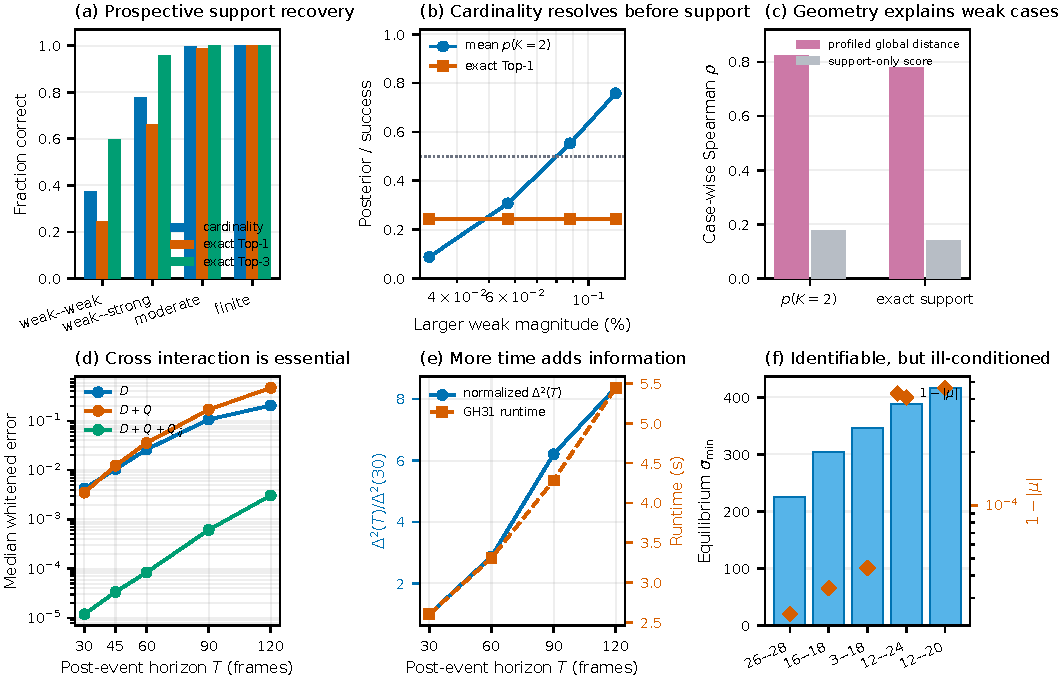
\includegraphics[width=\textwidth]{figures/generated/multi_event_evidence.pdf}
\caption{Why simultaneous-source recovery fails in the weak regime. Prospective results first separate cardinality from exact support (a--b). Retrospective geometry then links weak-case errors to profiled response distance (c). The longer-horizon diagnostic shows that the pairwise interaction is needed (d), information accumulates with time (e), and distinct equilibrium signatures can remain nearly collinear (f). Panels (c)--(f) explain the result but do not replace a prospective recovery test.}
\label{fig:multi-event-evidence}
\end{figure*}

Event presence is easier than source recovery. The frozen detector separates most event and no-event records, but its no-event exposure is too short for an operational false-alarm claim. Per-bus inclusion probabilities also rank useful candidates, yet their missed-source rate remains too high to repair weak exact-support decisions. Supplementary Appendix~G reports these secondary metrics and denominators.

\subsection{Profiled Geometry Explains the Weak Cases}

The retrospective audit asks why the weak bank fails. A support-only score compares candidate signatures while holding the rest of the explanation fixed. The profiled distance instead allows the competing support to choose its best amplitude and thereby measures the actual overlap between response manifolds. The latter tracks exact weak-case recovery far more closely [Fig.~\ref{fig:multi-event-evidence}(c)].

This result changes the interpretation of the weak regime. Every tested direction is first-order resolvable, so a curvature-dominated $a^{-4}$ delay law is not the observed mechanism. The errors arise because several finite-horizon candidate responses lie close after amplitude profiling. Detectability and source identity therefore require different geometric quantities.

The first-order theory separates two reasons for that proximity. A source may have
little response outside the nuisance span, or it may remain visible but nearly
collinear with another source after nuisance removal. Shared-source competitors
make the second mechanism especially severe because their common component
cancels before the exclusive source is compared. The frozen audit uses the full
nonlinear profiled distance and supports this explanation retrospectively; it does
not yet validate the analytic small-amplitude coefficient in
\eqref{eq:support-to-support-margin}.

The 120-frame diagnostic adds a second piece of the explanation. Extending the window increases the separation proxy by more than eightfold, and no candidate pair is exactly degenerate in the frozen equilibrium model. Yet the hardest signatures remain almost collinear [Fig.~\ref{fig:multi-event-evidence}(e)--(f)]. More time adds information without guaranteeing a well-conditioned decision.

The physical-manifold check also shows why the nonlinear interaction in \eqref{eq:load-multi-source-mean} cannot be dropped. Adding only single-source curvature does not improve the simultaneous response; adding $\bm Q_{ij}$ reduces the median whitened error by roughly two orders of magnitude [Fig.~\ref{fig:multi-event-evidence}(d)]. This check covers 32 nominal-operating-point paths. It validates the representation locally, not population recovery at 120 frames or robustness to operating shift.

\subsection{RQ4 Source Labels Do Not Generalize to New Assets}

The supervised hierarchy provides a useful contrast. On the ordinary split it detects events and ranks known sources well, confirming that multiscale dynamics, adaptive residuals, and PMU contrasts carry event information. That result answers interpolation at represented assets.

The source-holdout result answers a different question. With the physical asset removed from all source-labeled fitting and the true event family supplied, only \HeldSourceCorrect{} of \HeldSourceDecisions{} decisions are exact. The failure remains after detection and family confusion have been removed. The location heads and asset descriptors therefore memorize source-specific associations that do not transfer to an unseen physical source.

The physical load bank avoids that shortcut by generating a response for every candidate support. Its success is narrower in another direction: it covers only load interventions under fixed topology, known onset, matched operation, and synthetic noise. Together, the two experiments motivate the next model rather than a claim of general superiority: learned residuals should correct a physical candidate likelihood and must be tested on event parents and source assets excluded from training.

\section{Discussion and Limitations}
\label{sec:discussion}

The two simulators expose different parts of the inverse problem. Eight voltage/current PMUs recover the requested 31-bus voltage field accurately in the PowerDynamics tests even though the 114-state local model is not fully observable. The same sensor buses support reliable abnormal-event detection and moderate known-source localization in ANDES. Neither result transfers to the other task. Low hidden-voltage HVRE does not guarantee source separation, and high detection F1 does not identify a hidden state or a physical source.

The local theory explains this split. Proposition~\ref{prop:functional-reconstruction} removes unobservable directions that do not affect the requested voltage function. Corollary~\ref{cor:functional-blue} then attaches a covariance to that estimable function; rank alone cannot provide it. Source diagnosis has a different geometry. Proposition~\ref{prop:source-indistinguishability} tests whether two candidate-nuisance response sets intersect, while Proposition~\ref{prop:nonlinear-separation} requires the affine distance to exceed the combined DAE remainder before local nonlinear separation is certified. Large faults, topology switches, and unmodeled controls may violate the neighborhood in which that bound holds.

Only the first theory-to-data link has been tested. The preregistered functional residual correlates with bus-level error, although excitation, scaling, estimator covariance, and electrical distance explain several exceptions. The source-held-out failure is compatible with poor physical separation, source memorization, or both. The current artifacts cannot separate those explanations. Computing \eqref{eq:pairwise-information} before model fitting and relating it to held-source errors would test the mechanism directly.

The operating-point study also separates target recovery from parameter recovery. Regularized physical recentering closes \EZeroHClosureOverall{} of the oracle-center gap on M6 although only \EZeroHRank{} of \EZeroHDimension{} nuisance directions are locally informed. The hidden-voltage target can therefore be accurate while the injection coordinates remain non-unique. This result is confined to an equilibrium snapshot. It does not cover line outages, faults, or sequential event-conditioned estimation, and the local curvature covariance remains under-dispersed in the joint NEES-like statistic.

The legacy event model supplies one reusable mechanism and one clear warning. Multiscale summaries, adaptive residuals, and simultaneous PMU contrasts improve known-source physical ranking by \LegacyPhysicalGainPP{} percentage points. Availability belongs in the integrity state because a missing measurement is observed directly. Source identities and endpoint descriptors, however, allow memorization. Exact localization falls to \HeldSourceRate{} under complete physical-source holdout. A source-generalizable model should instead compute engineered features from candidate residuals, $\bm y-\widehat{\bm y}_h$, and compare their contribution with a physics-only likelihood.

The principal evidence gap is the absence of one end-to-end experiment. The state and event studies use different simulators, measurement semantics, and split rules. Both are simulated; neither supplies field or hardware-in-the-loop validation. The event records also have fixed onsets and only about 7.15~min of normal-labeled exposure per split, too little for an operational false-alarm rate. PMU loss and addition have not been linked prospectively to the separation margin, and the candidate posterior has not been calibrated.

A decisive follow-up requires one audited plant and measurement operator for learned-only, physics-only, learned-residual, and diagnosability-aware methods. Event parents and physical sources must be disjoint across fitting, calibration, and test. Operating-point shift, parameter error, and PMU loss or addition should be imposed before the test is opened. A long normal stream must report false alarms per hour and event recall; event-source correctness, candidate-set coverage, resolution delay, HVRE, calibration error, runtime, and failed solves complete the evaluation. Without that experiment, joint superiority remains unproved.

\section{Conclusion}
\label{sec:conclusion}

We formulated sparse PMU event diagnosis as inference over physical interventions observed through a time-varying, integrity-aware measurement network. The manuscript connects PMU-projected source separation, causal Bayesian evidence, candidate sets, and model-mediated knowledge transfer, while preserving explicit abstention when exact localization is not justified. The next scientific step is not to fill this structure with plausible numbers; it is to execute and freeze the four experimental campaigns that determine which of these proposed capabilities hold under source exclusion, PMU membership changes, simulator transfer, and continuous scanning.


% Acknowledgments and author biographies are intentionally omitted until author-provided.
\bibliographystyle{IEEEtran}
\bibliography{references}

\EOD
\end{document}
